\section{Binary files}

Binary formats contain vital information regarding a file's organization on disk, memory loading procedures, file type, machine class, and sections. 
ELF (Executable and Linkable Format) binaries adhere to the following structure:
\begin{itemize}
    \item \textit{ELF header}: this component delineates the overarching structure of the binary, specifying the file type and demarcating the boundaries for section and program headers.
    \item \textit{Program headers}: these headers explain how the file will be loaded into memory. 
        They segment the data into distinct parts and establish mappings between sections and segments.
    \item \textit{Section headers}: these headers provide a representation of the binary as it exists on disk, defining various sections, including:
        \begin{itemize}
            \item \texttt{.init}: contains executable instructions responsible for initializing the process.
            \item \texttt{.text}: holds the executable instructions of the program.
            \item \texttt{.bss}: reserved for statically-allocated variables.
            \item \texttt{.data}: reserved for initialized data.
        \end{itemize}
\end{itemize}

\paragraph*{Segment}
Segments represent the runtime view of a binary. 
They define how the binary will be loaded into memory, dividing the data into distinct segments and specifying the mapping between sections and segments. 
Segments play a crucial role in the execution of the program by providing the necessary information for the operating system to allocate memory and execute the binary.

\paragraph*{Section}
Sections in an ELF binary contain linking and relocation information. 
They provide granular details about the various components of the binary, such as code, data, and symbols.
Sections are essential for the linking process, aiding in resolving external symbols and determining memory layout. 
They also facilitate relocation, enabling the binary to be loaded and executed correctly in different memory locations. 
Sections serve as the building blocks for the organization and structure of the ELF binary.

\subsection{Linux processes}
\paragraph*{Creation}
When a program is executed in Linux, it undergoes a series of steps to be mapped into memory and organized for execution:
\begin{enumerate}
    \item \textit{Creation of virtual address space}: the kernel initiates by creating a virtual address space dedicated to the program's execution, providing isolation and abstraction.
    \item \textit{Loading information from executable file}: the kernel, with the assistance of the dynamic linker, loads relevant information from the executable file into the newly allocated address space. 
        This process involves loading the segments specified by the program headers of the ELF binary.
    \item \textit{Setup of stack and heap}: after loading the necessary information, the kernel sets up the stack and heap within the program's address space. 
        The kernel then initiates execution by jumping to the designated entry point of the program.
\end{enumerate}
\begin{figure}[H]
    \centering
    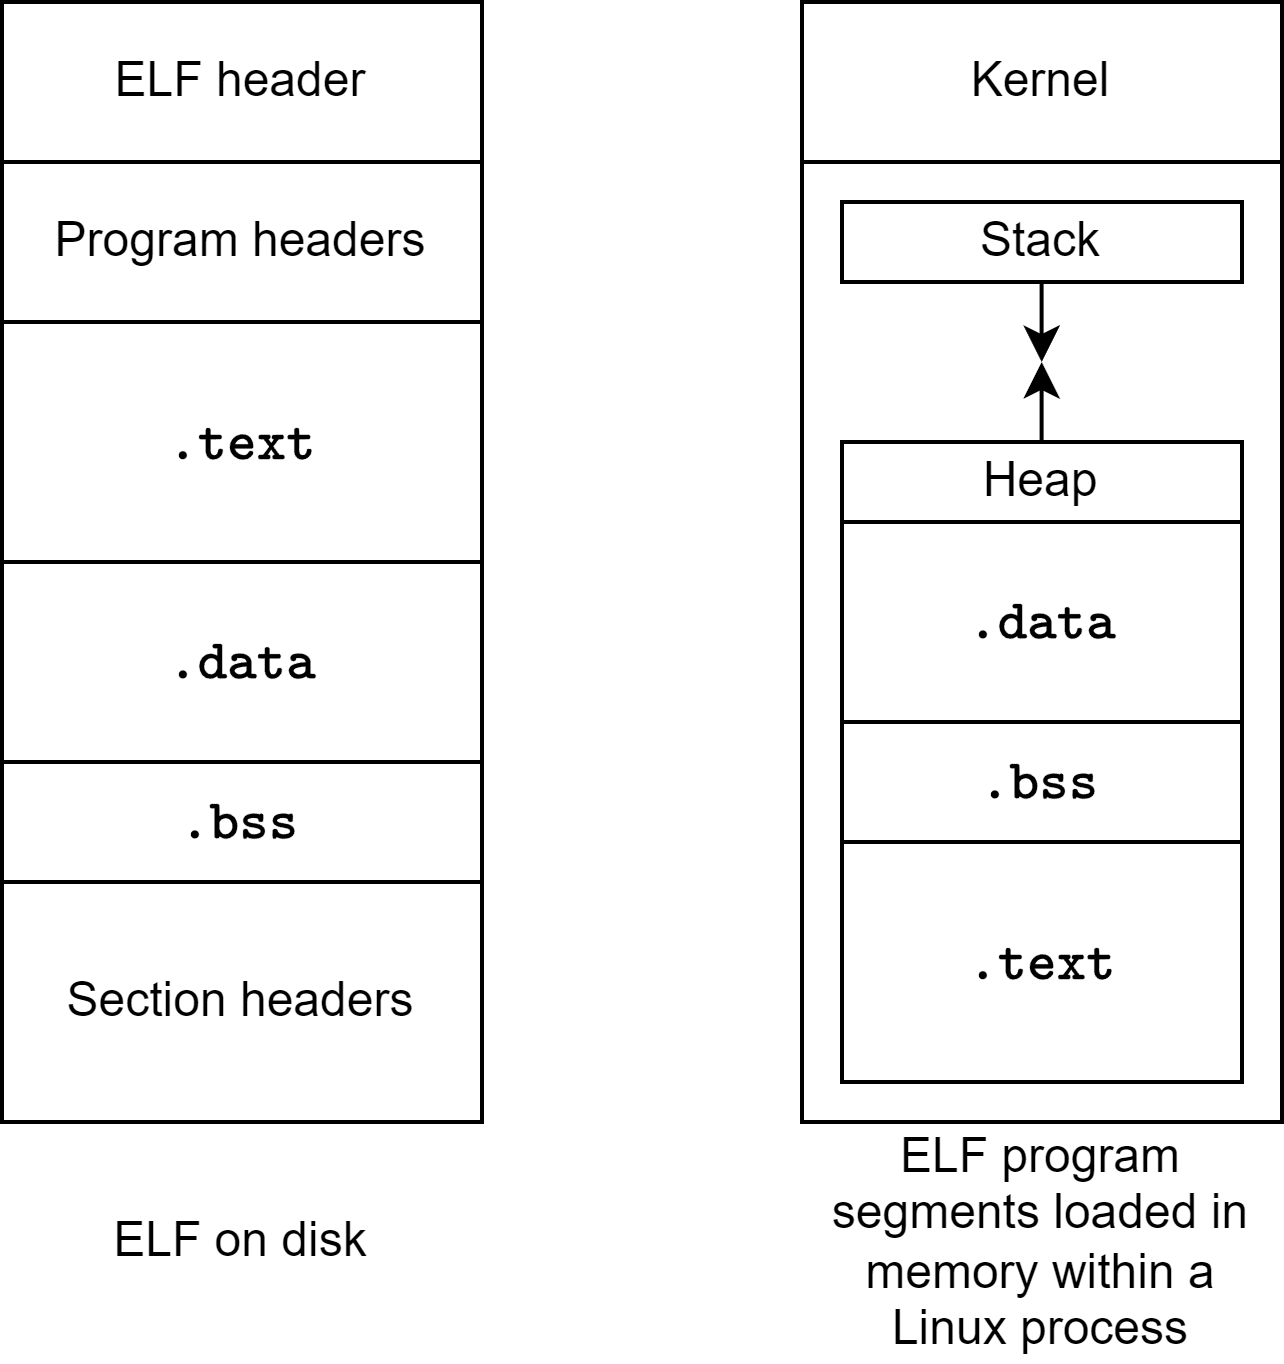
\includegraphics[width=0.4\linewidth]{images/linux.png}
    \caption{Process layout in Linux}
\end{figure}

\paragraph*{Execution}
Once a program is correctly created, the virtual address space contains the following elements:
\begin{itemize}
    \item \textit{Argc, env pointer, and stack}: this region includes statically allocated local variables, environment variables, and function activation records.
        The stack grows downward, towards lower addresses, as more function calls and local variables are added.
    \item \textit{Unallocated memory}.
    \item \textit{Heap}: dynamically allocated data resides in this section. 
        The heap grows upward, towards higher addresses, as more memory is dynamically allocated during program execution.
    \item \texttt{.data}, \texttt{.bss}, and \texttt{.text}. 
    \item \textit{Shared libraries}. 
\end{itemize}
\begin{figure}[H]
    \centering
    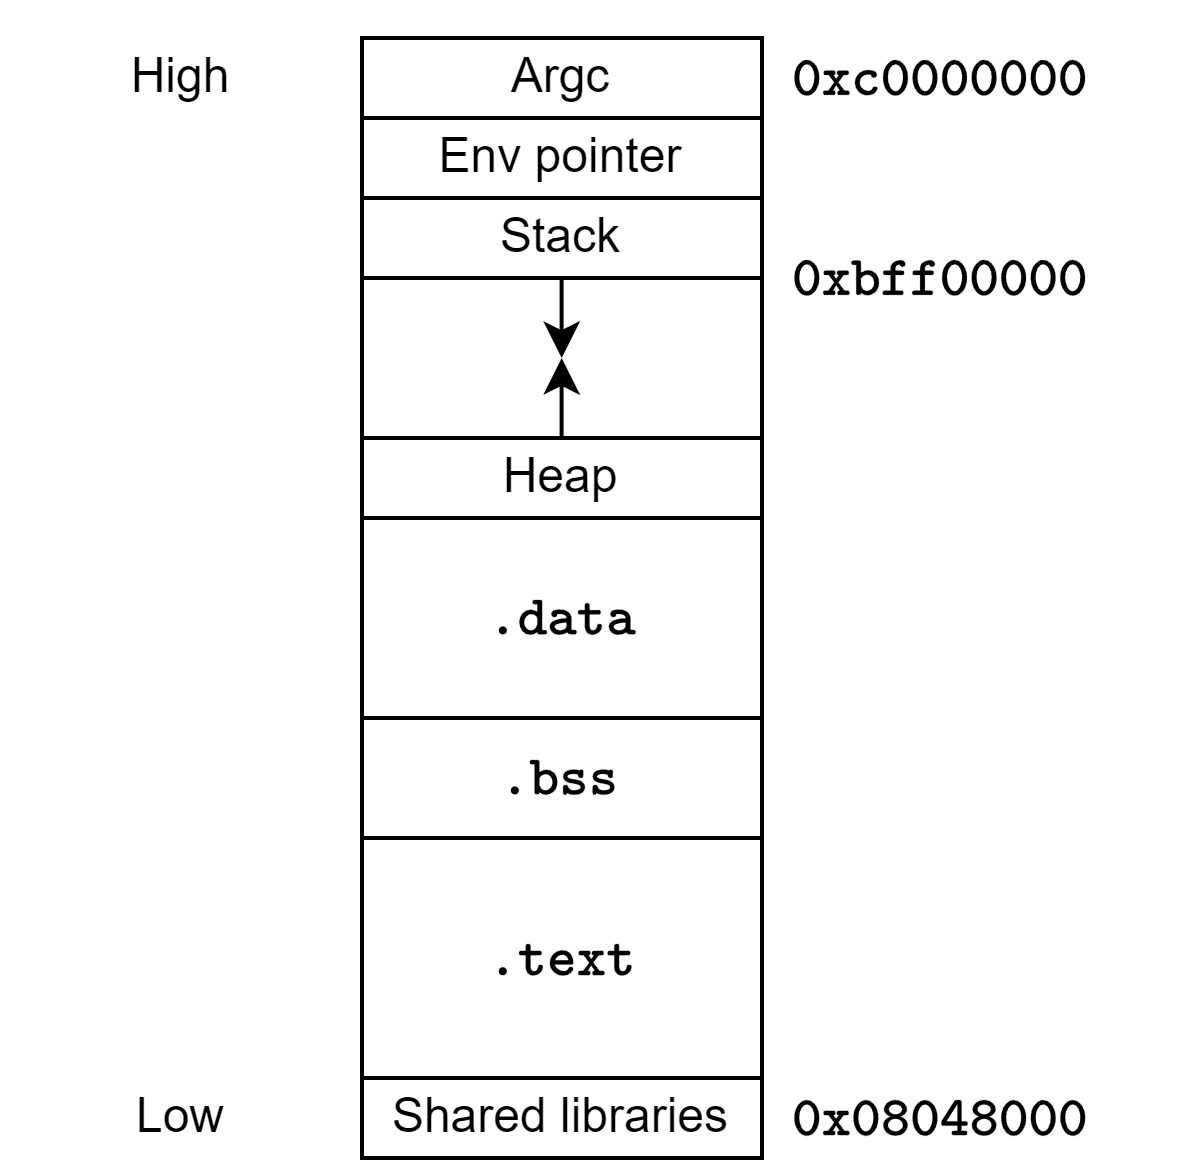
\includegraphics[width=0.4\linewidth]{images/stack.png}
    \caption{Code structure}
\end{figure}

\paragraph*{Termination}
When the program completes its execution, the CPU needs to determine where to jump next. 
Typically, after a function finishes executing, the control flow returns to the point in the program from which the function was called. 
This return address is crucial for maintaining the program's execution flow.

To achieve this, the CPU saves the current instruction pointer (EIP) onto the stack before jumping to the called function. 
When the function completes its execution, the CPU retrieves the return address from the stack and jumps to that address, resuming execution from the point where the function was initially called.